%% Преамбула TeX-файла

% 1. Стиль и язык
\documentclass[utf8x, 12pt]{G7-32} % Стиль (по умолчанию будет 14pt)

% Остальные стандартные настройки убраны в preamble.inc.tex.
\sloppy

% Настройки стиля ГОСТ 7-32
% Для начала определяем, хотим мы или нет, чтобы рисунки и таблицы нумеровались в пределах раздела, или нам нужна сквозная нумерация.
\EqInChapter % формулы будут нумероваться в пределах раздела
\TableInChapter % таблицы будут нумероваться в пределах раздела
\PicInChapter % рисунки будут нумероваться в пределах раздела
\usepackage{slashbox}

% Добавляем гипертекстовое оглавление в PDF
\usepackage[
bookmarks=true, colorlinks=true, unicode=true,
urlcolor=black,linkcolor=black, anchorcolor=black,
citecolor=black, menucolor=black, filecolor=black,
]{hyperref}

% Изменение начертания шрифта --- после чего выглядит таймсоподобно.
% apt-get install scalable-cyrfonts-tex

\IfFileExists{cyrtimes.sty}
    {
        \usepackage{cyrtimespatched}
    }
    {
        % А если Times нету, то будет CM...
    }

\usepackage{graphicx}   % Пакет для включения рисунков

% С такими оно полями оно работает по-умолчанию:
% \RequirePackage[left=20mm,right=10mm,top=20mm,bottom=20mm,headsep=0pt]{geometry}
% Если вас тошнит от поля в 10мм --- увеличивайте до 20-ти, ну и про переплёт не забывайте:
\geometry{right=20mm}
\geometry{left=30mm}


% Пакет Tikz
\usepackage{tikz}
\usetikzlibrary{arrows,positioning,shadows}

% Произвольная нумерация списков.
\usepackage{enumerate}

% ячейки в несколько строчек
\usepackage{multirow}

% itemize внутри tabular
\usepackage{paralist,array}

% Центрирование подписей к плавающим окружениям
\usepackage[justification=centering]{caption}


% Настройки листингов.
\ifPDFTeX
% 8 Листинги

\usepackage{listings}
\usepackage{wrapfig}
% Значения по умолчанию
\lstset{
  basicstyle= \footnotesize,
  breakatwhitespace=true,% разрыв строк только на whitespacce
  breaklines=true,       % переносить длинные строки
%   captionpos=b,          % подписи снизу -- вроде не надо
  inputencoding=koi8-r,
  numbers=left,          % нумерация слева
  numberstyle=\footnotesize,
  showspaces=false,      % показывать пробелы подчеркиваниями -- идиотизм 70-х годов
  showstringspaces=false,
  showtabs=false,        % и табы тоже
  stepnumber=1,
  tabsize=4,              % кому нужны табы по 8 символов?
  frame=single
}

% Стиль для псевдокода: строчки обычно короткие, поэтому размер шрифта побольше
\lstdefinestyle{pseudocode}{
  basicstyle=\small,
  keywordstyle=\color{black}\bfseries\underbar,
  language=Pseudocode,
  numberstyle=\footnotesize,
  commentstyle=\footnotesize\it
}

% Стиль для обычного кода: маленький шрифт
\lstdefinestyle{realcode}{
  basicstyle=\scriptsize,
  numberstyle=\footnotesize
}

% Стиль для коротких кусков обычного кода: средний шрифт
\lstdefinestyle{simplecode}{
  basicstyle=\footnotesize,
  numberstyle=\footnotesize
}

% Стиль для BNF
\lstdefinestyle{grammar}{
  basicstyle=\footnotesize,
  numberstyle=\footnotesize,
  stringstyle=\bfseries\ttfamily,
  language=BNF
}

% Определим свой язык для написания псевдокодов на основе Python
\lstdefinelanguage[]{Pseudocode}[]{Python}{
  morekeywords={each,empty,wait,do},% ключевые слова добавлять сюда
  morecomment=[s]{\{}{\}},% комменты {а-ля Pascal} смотрятся нагляднее
  literate=% а сюда добавлять операторы, которые хотите отображать как мат. символы
    {->}{\ensuremath{$\rightarrow$}~}2%
    {<-}{\ensuremath{$\leftarrow$}~}2%
    {:=}{\ensuremath{$\leftarrow$}~}2%
    {<--}{\ensuremath{$\Longleftarrow$}~}2%
}[keywords,comments]

% Свой язык для задания грамматик в BNF
\lstdefinelanguage[]{BNF}[]{}{
  morekeywords={},
  morecomment=[s]{@}{@},
  morestring=[b]",%
  literate=%
    {->}{\ensuremath{$\rightarrow$}~}2%
    {*}{\ensuremath{$^*$}~}2%
    {+}{\ensuremath{$^+$}~}2%
    {|}{\ensuremath{$|$}~}2%
}[keywords,comments,strings]

% Подписи к листингам на русском языке.
\renewcommand\lstlistingname{\cyr\CYRL\cyri\cyrs\cyrt\cyri\cyrn\cyrg}
\renewcommand\lstlistlistingname{\cyr\CYRL\cyri\cyrs\cyrt\cyri\cyrn\cyrg\cyri}

\else
\usepackage{local-minted}
\fi
\usepackage{dirtytalk}
\usepackage{algorithm2e}
\usepackage[noend]{algpseudocode}
\usepackage{csquotes}
\usepackage[at]{easylist}
\usepackage{pgfplots}

% Полезные макросы листингов.
% Любимые команды
\newcommand{\Code}[1]{\textbf{#1}}


\begin{document}

\frontmatter % выключает нумерацию ВСЕГО; здесь начинаются ненумерованные главы: реферат, введение, глоссарий, сокращения и прочее.

% Команды \breakingbeforechapters и \nonbreakingbeforechapters
% управляют разрывом страницы перед главами.
% По-умолчанию страница разрывается.

% \nobreakingbeforechapters
% \breakingbeforechapters

% НАЧАЛО ТИТУЛЬНОГО ЛИСТА
\begin{center}
	\hfill \break
	\textit{
		\normalsize{Государственное образовательное учреждение высшего профессионального образования}}\\ 
	
	\textit{
		\normalsize  {\bf  «Московский государственный технический университет}\\ 
		\normalsize  {\bf имени Н. Э. Баумана»}\\
		\normalsize  {\bf (МГТУ им. Н.Э. Баумана)}\\
	}
	\noindent\rule{\textwidth}{2pt}
	\hfill \break
	\noindent
	\\
	\noindent
	\\
	\hfill\break
	\hfill \break
	\hfill \break
	\hfill \break
	
	\hfill \break
	\large{Лабораторная работа №1\\ \textquote{Расстояние Левенштейна}}\\
	\hfill \break
	\hfill \break
	\hfill \break
	\hfill \break
	\hfill \break	
	\normalsize {
		\begin{minipage}[t]{7cm}
		\end{minipage}
		\hfill
		\begin{minipage}[t]{7cm}
			\flushright
			Студент: Камакин А.С.\\
			Группа: ИУ7-53\\
			Преподаватель: Волкова Л.Л.
		\end{minipage}
	}\\
	\hfill \break	
	\hfill \break
	\hfill \break
	\hfill \break
	\hfill \break
\end{center}
\hfill \break
\hfill \break
\begin{center} Москва 2017 \end{center}

\thispagestyle{empty} % 
% КОНЕЦ ТИТУЛЬНОГО ЛИСТА

\newpage
% \tableofcontents

\mainmatter % это включает нумерацию глав и секций в документе ниже

Введём модель вычисления, используемую при оценках трудоёмкости:
\begin{itemize}
	\item вызов метода объекта структуры имеет трудоёмкость 1;
	\item объявление переменной/массива/структуры без определения имеет трудоёмкость 0;
	\item операторы $+$, $-$, $*$, $/$, $=$, $++$, $--$ имеют трудоёмкость 1;
	\item условный оператор (без условий внутри) имеет трудоёмкость 0;
	\item логические операции имеют трудоёмкость 1; 
	\item оператор цикла имеет трудоёмкость $1 + n(3 + T)$, где $n$ – это число повторений цикла, $T$ – трудоёмкость тела цикла;
	\begin{itemize}
		\item \textbf{Замечание:} так как доподлинно неизвестно, каким образом компилятор интерпретирует цикл, целесообразно взять модель, предложенную на преподавателем: одно присваивание до цикла (1 операция), внутри цикла присваивание, сравнение и инкремент (3 операции).
	\end{itemize}
	\item вызов функции имеет трудоёмкость 0, так как функции компилятор рассматривает как inline и подставляет сразу вместо вызова код.
	\item $Fn(n)$ – часть трудоёмкости, зависящая только от размера входа;
	\item $g(D)$ – часть трудоёмкости, зависящая от конкретного входа, значений переменных.
\end{itemize}

\newpage

\paragraph{Итеративный алгоритм для расстояния Левенштейна}
\begin{center}
	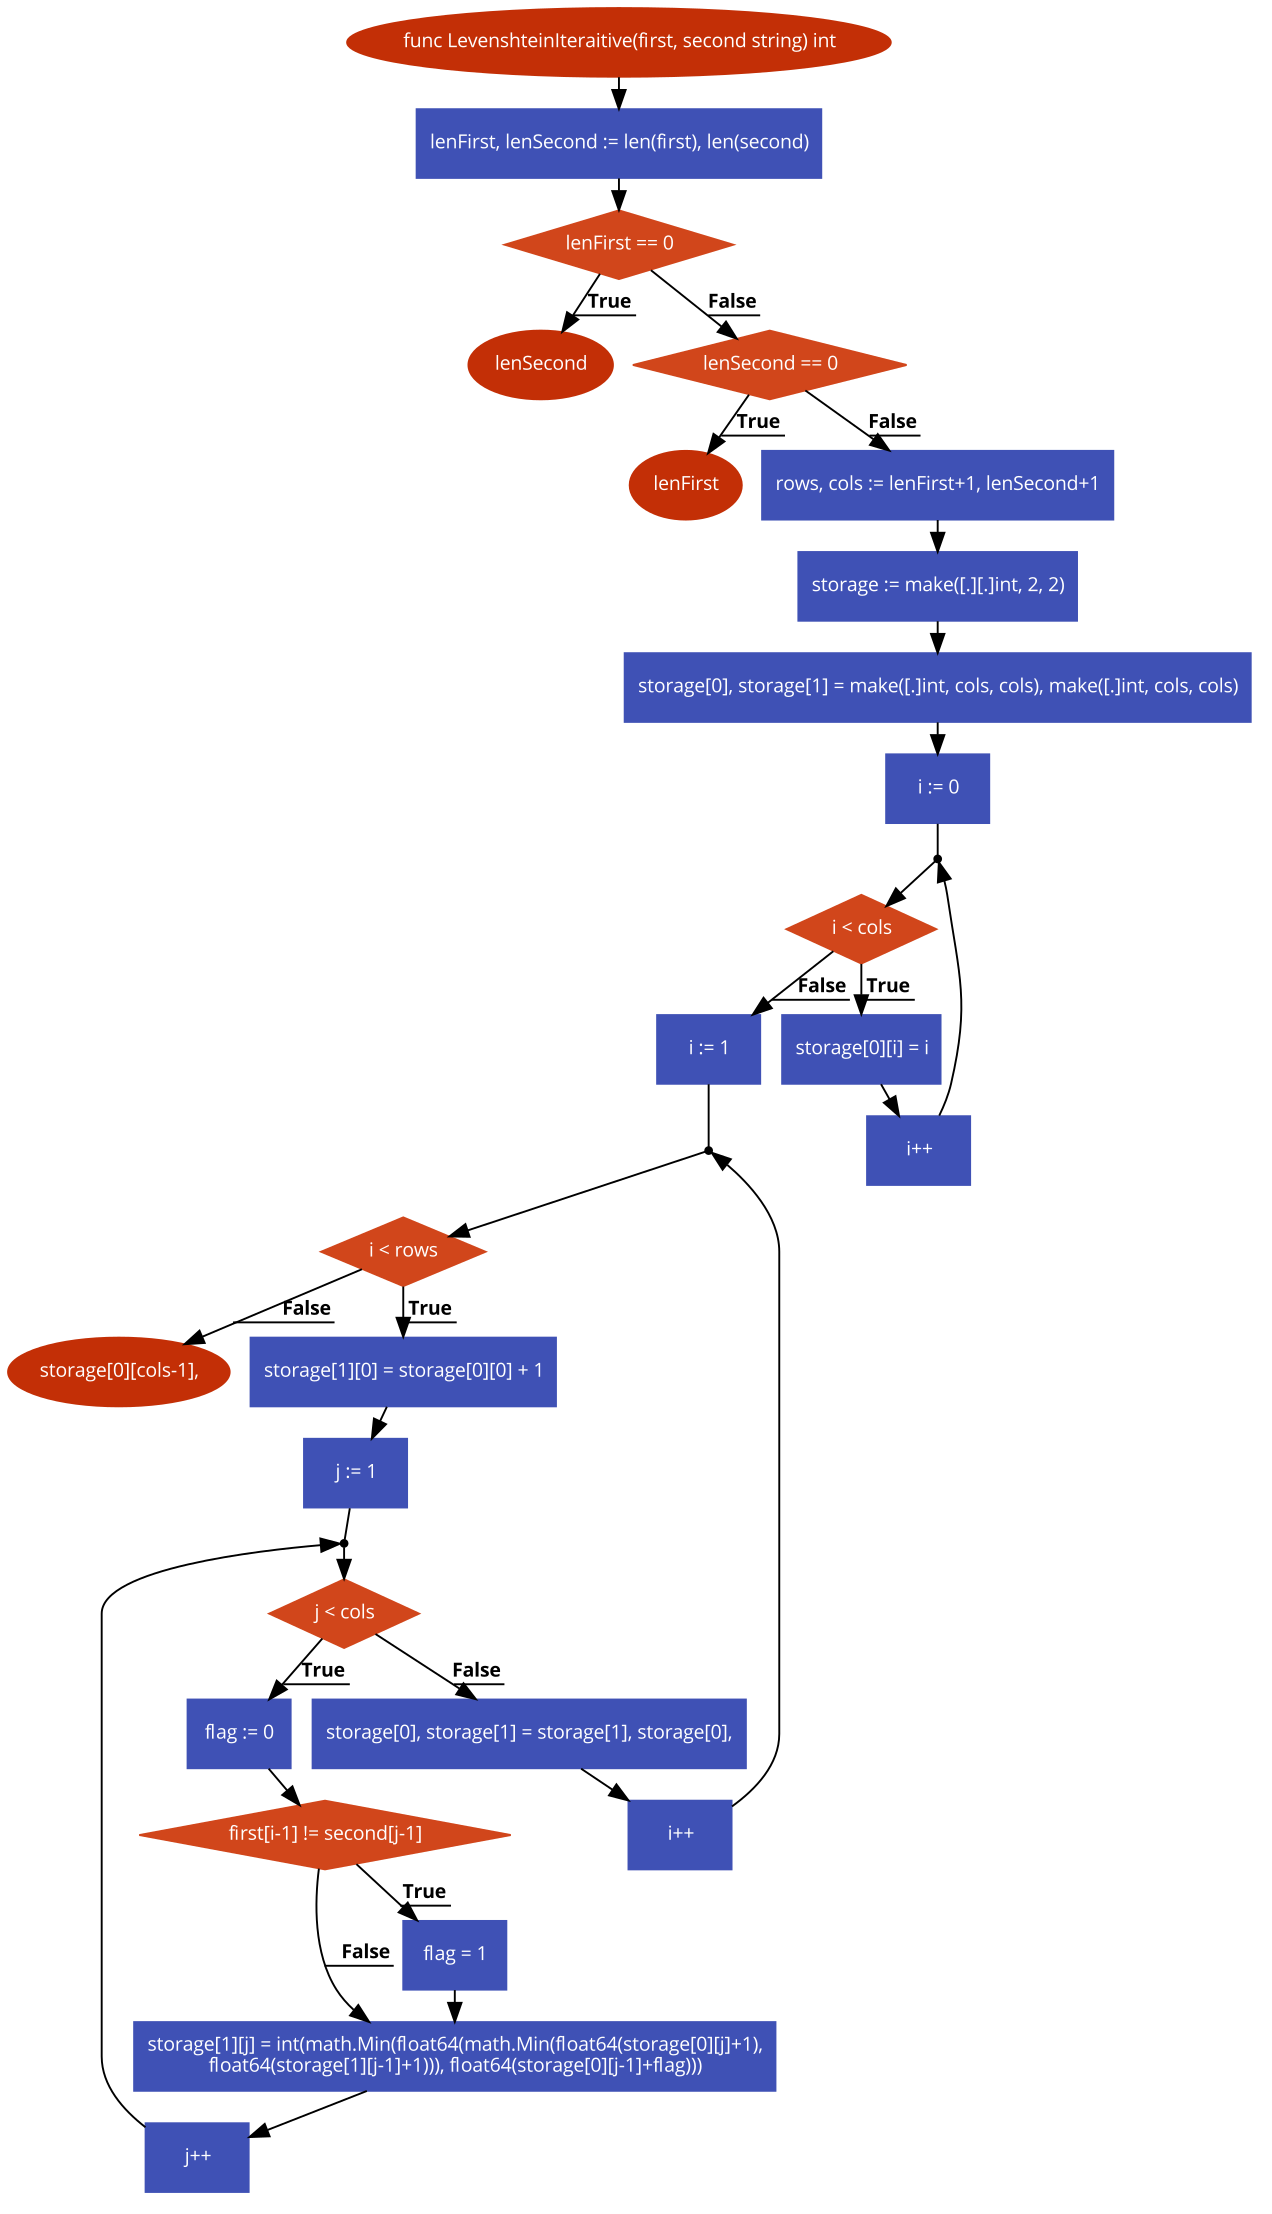
\includegraphics[scale=0.32]{images/levenshteinIterative.png}
\end{center}

\newpage

\paragraph{Рекурсивный алгоритм для расстояния Левенштейна}
\begin{center}
	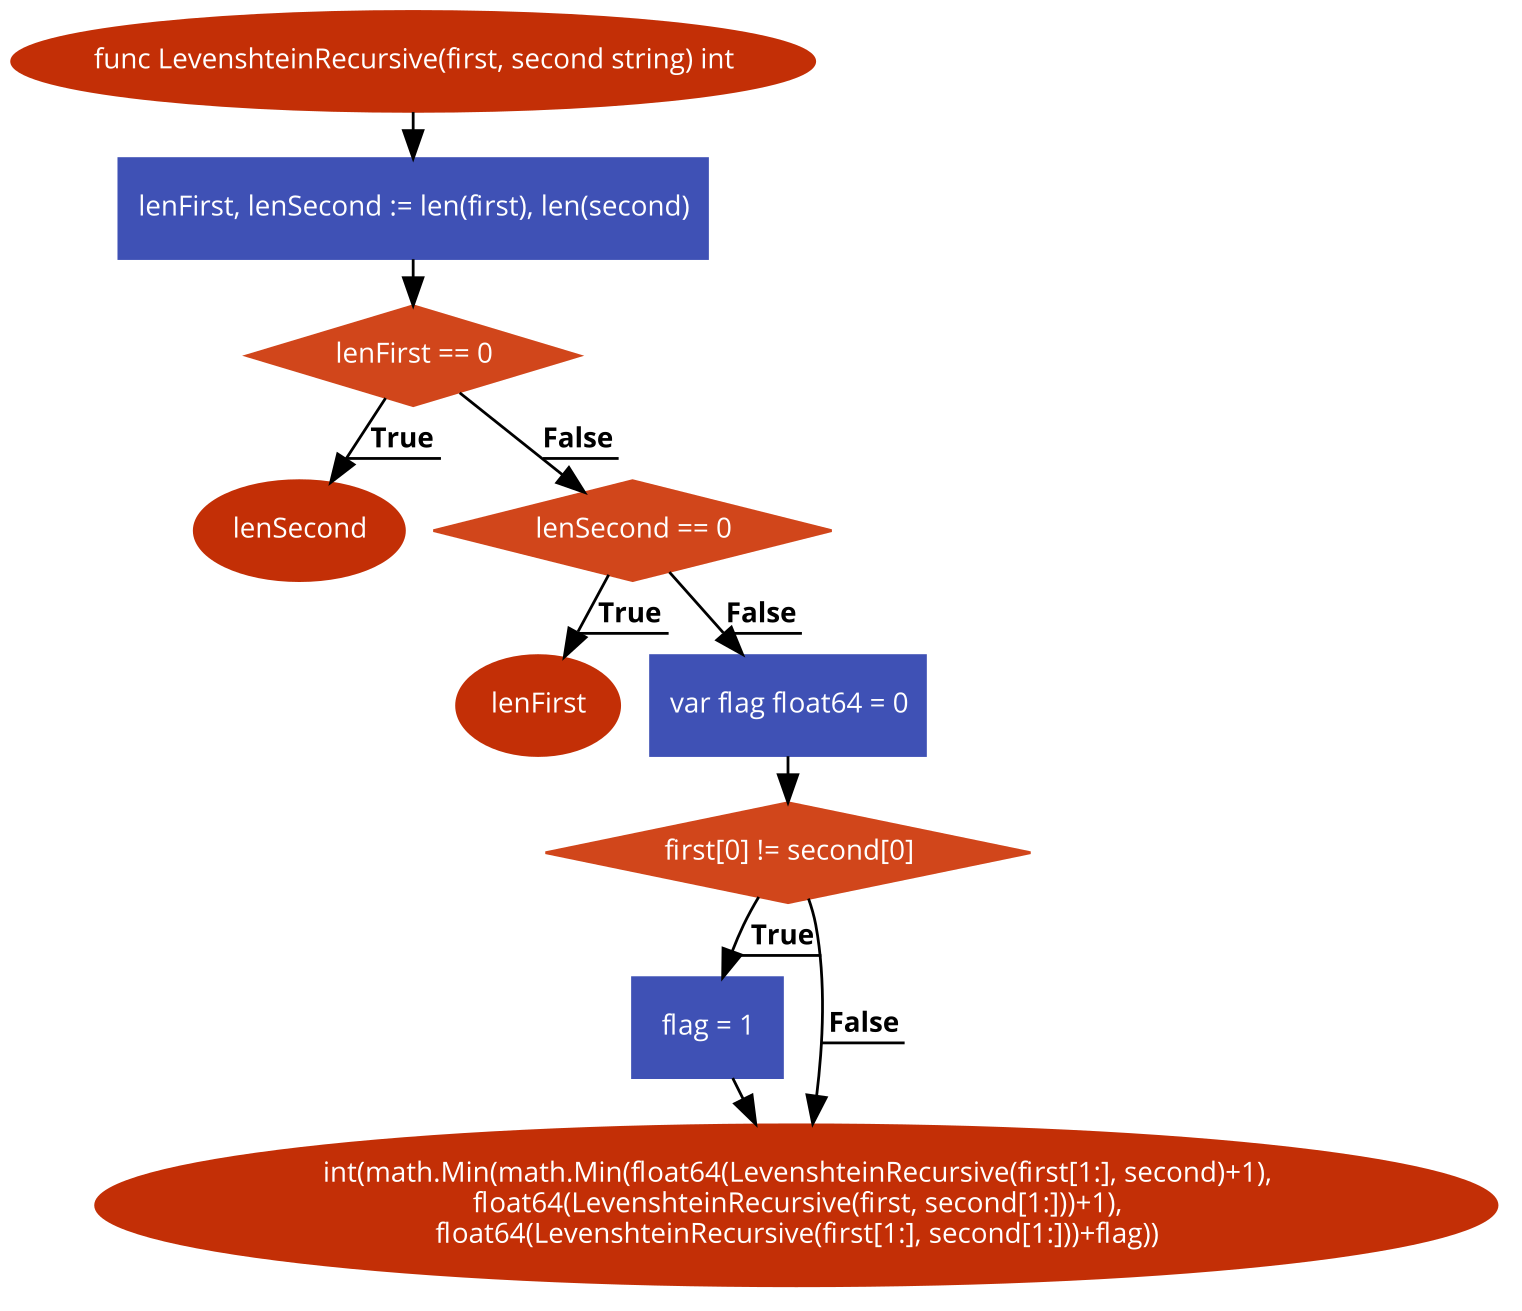
\includegraphics[scale=0.32]{images/levenshteinRecursive.png}
\end{center}

\newpage

\paragraph{Модифицированный алгоритм для расстояния Левенштейна}
\begin{center}
	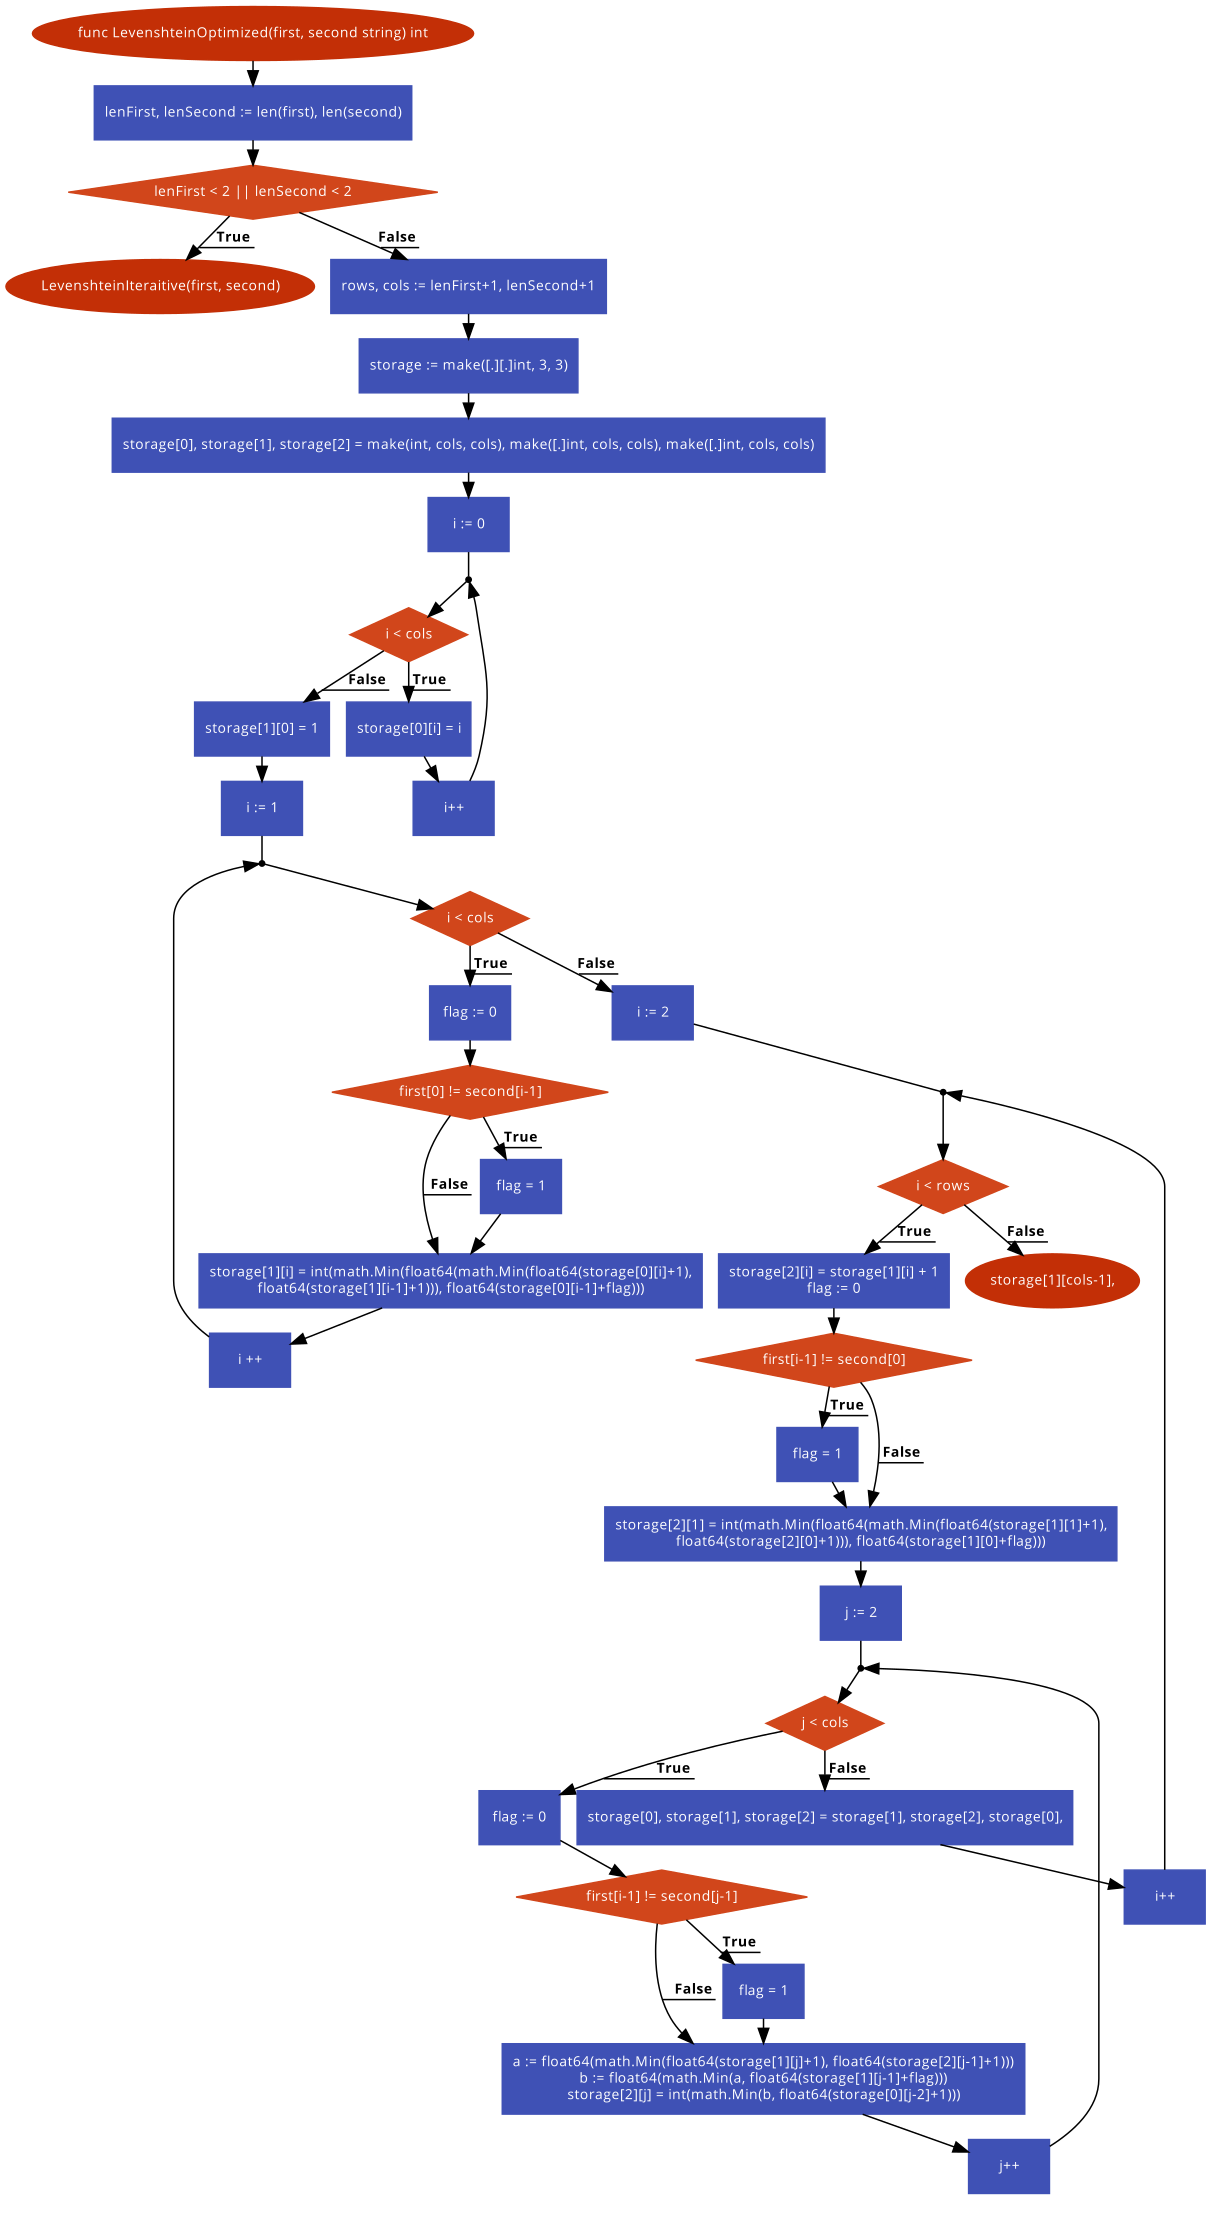
\includegraphics[scale=0.32]{images/levenshteinOptimized.png}
\end{center}

\newpage

\paragraph{Графики}
\begin{center}
\begin{tikzpicture}
\begin{axis}[
title={Сравнение работы алгоритмов по времени (gobench)},
xlabel={длина строки $l$},
ylabel={время $t(ns)$},
xmin=0, xmax=140,
ymin=0, ymax=370000,
xtick={0,20,40,60,80,100,120, 140},
ytick={0,50000,100000,150000,200000,250000,300000,350000},
legend pos=north west,
ymajorgrids=true,
grid style=dashed,
]

\addplot[
color=blue,
mark=square,
]
coordinates {
	(2,173)(4,377)(8,1202)(16,4532)(32,16822)(64,65381)(128,263032)
};
\addlegendentry{итеративный}

\addplot[
color=red,
mark=star,
]
coordinates {
	(2,143)(4,3892)(8,3126165)
};
\addlegendentry{рекурсивный}

\addplot[
color=green,
mark=triangle,
]
coordinates {
	(2,183)(4,420)(8,1438)(16,5860)(32,22409)(64,87776)(128,352257)
};
\addlegendentry{модифицированный}

\end{axis}
\end{tikzpicture}
\end{center}

\begin{center}
	\begin{tikzpicture}
	\begin{axis}[
	title={Сравнение работы алгоритмов по количеству итераций за время $t_0$ (gobench)},
	xlabel={длина строки $l$},
	ylabel={количество итераций за $t_0$},
	xmin=0, xmax=140,
	ymin=0, ymax=10000000,
	xtick={0,20,40,60,80,100,120, 140},
	ytick={0,2000000,4000000,6000000,8000000,10000000},
	legend pos=north west,
	ymajorgrids=true,
	grid style=dashed,
	]
	
	\addplot[
	color=blue,
	mark=square,
	]
	coordinates {
		(2,10000000)(4,5000000)(8,1000000)(16,300000)(32,100000)(64,20000)(128,5000)
	};
	\addlegendentry{итеративный}
	
	\addplot[
	color=red,
	mark=star,
	]
	coordinates {
		(2,10000000)(4,300000)(8,500)
	};
	\addlegendentry{рекурсивный}
	
	\addplot[
	color=green,
	mark=triangle,
	]
	coordinates {
		(2,10000000)(4,3000000)(8,1000000)(16,300000)(32,100000)(64,20000)(128,5000)
	};
	\addlegendentry{модифицированный}
	
	\end{axis}
	\end{tikzpicture}
\end{center}

\newpage

\paragraph{Тестовые данные}\\

Время работы в наносекундах (ns):\\

\begin{tabular}{l*{7}{c}r}
	Алгоритм & 2 & 4 & 8 & 16 & 32 & 64 & 128 \\
	\hline
	Итеративный & 173 & 377 & 1202 & 4532 & 16822 & 65381 & 263032 \\
	Рекурсивный & 143 & 3892 & 3126165 & - &  - & - & - \\
	Модифицированный & 183 & 420 & 1438 & 5860 & 22409 & 87776 & 352257 \\
\end{tabular}\\\\

Количество итераций за время $t_0$:\\

\begin{tabular}{l*{7}{c}r}
	Алгоритм & 2 & 4 & 8 & 16 & 32 & 64 & 128 \\
	\hline
	Итеративный & 10000000 & 5000000 & 1000000 & 300000 & 100000 & 20000 & 5000 \\
	Рекурсивный & 10000000 & 300000 & 500 & - &  - & - & - \\
	Модифицированный & 10000000 & 3000000  & 1000000 & 300000 & 100000 & 20000 & 5000 \\
\end{tabular}

\newpage

\paragraph{Оценка трудоемкостей алгоритмов}
\begin{enumerate}
	\item Итеративный алгоритм: $9 + c(3 + 1) + r(3 + 2 + c(3 + 2 + 
	\begin{cases}
	1,& \text{if true}\\
	0,& \text{otherwise}
	\end{cases}
	 + 6) + 2)$
	\begin{itemize}
		\item при выполнении условия: $9 + 4c + 7r + 12rc$
		\item при невыполнении условия: $9 + 4c + 7r + 11rc$
	\end{itemize}
	\item Рекурсивный алгоритм: $4 + 
	\begin{cases}
	1,& \text{if true}\\
	0,& \text{otherwise}
	\end{cases}
	+ 3^n$
	\begin{itemize}
		\item при выполнении условия: $5 + 3^n$
		\item при невыполнении условия: $4 + 3^n$
	\end{itemize}
	\item Модифицированный алгоритм: $11 + c(3 + 1) + 1 + (c - 1)(5 + \begin{cases} 1,& \text{if true}\\0,& \text{otherwise}\end{cases} + 3) + (r - 2)(7 + \begin{cases} 1,& \text{if true}\\0,& \text{otherwise}\end{cases} + 6 + (c - 2)(5 + \begin{cases} 1,& \text{if true}\\0,& \text{otherwise}\end{cases} + 10) + 3) \simeq $
	\begin{center}
		$36 - 16r - 18c + 15rc$
	\end{center}
\end{enumerate}

\paragraph{Заключение}

В ходе работы были описаны и реализованы различные варианты алгоритма Левенштейна (итеративный, рекурсивный и модифицированный), и был проведен сравнительный анализ их временной эффективности.

\backmatter %% Здесь заканчивается нумерованная часть документа и начинаются ссылки и
            %% заключение

\appendix   % Тут идут приложения

\end{document}

%%% Local Variables:
%%% mode: latex
%%% TeX-master: t
%%% End: